\chapter{Decidability Problems for Hinged Polygons and Disks}
\subsection{The Logic Engine}
\subsubsection{Construction of the Logic Engine and Encoding of an NAE3SAT Problem on a Logic 
Engine}
\begin{figure}[!h]
\begin{center}
%%%First Figure with armatures
\includegraphics{graphics/LogicEngineFrameFigure1Scaled.pdf}
\caption{A logic engine frame with veritical armatures and a horizontal 
shaft.}\label{fig:LogicEngineFrameFigure1.pdf}
\end{center}
\end{figure}
The logic engine is a physical model which can encode instances of the NAE3SAT problem.  The 
components of the logic engine are as follows: the rigid frame, the shaft, the armatures,
the chains, and the flags.  Figure \ref{fig:LogicEngineFrameFigure1.pdf} shows the a rigid frame, 
armatures, and shaft.  Each armature represents a boolean variable.  The rigid frame defines the border 
of the model and the armatures can rotate about the shaft.
\begin{figure}[!h]
\begin{center}
\includegraphics{graphics/LogicEngineFrameFigure2Scaled.pdf}
\caption{}\label{fig:LogicEngineFrameFigure2.pdf}
\end{center}
\end{figure}
Flagging arragement indicates the relationship of the boolean literal's existence within a clause.  There are two literals for each variable.  
\begin{enumerate}
 \item If the literal $x_j$ is found in clause $C_k$, then $l_{j,k}$ is unflagged.
 \item If the literal $\bar{x}_j$ is found in clause $C_k$, then $\bar{l}_{j,k}$ is unflagged.
\end{enumerate}
Negated literals reside below the shaft and non-negated literals reside above the shaft.
% If the NAE3SAT problem contains $m$ clauses, each armature is partitioned into $2m$ pieces.  Since the armatures represent the boolean variables, the corresponding l  $m$ pieces above the shaft and $m$ pieces below the shaft.  Each row at height $h$ above and below the shaft represents the $h^\text{th}$ clause in the boolean formula.  The flags indicate that the literal of the boolean variable does not occur in the clause, i.e.

A \textit{collision} of flags occur if either of the following occurs:
\begin{enumerate}
\item flags in the same row on adjacent armatures point toward each other.
\item a flag from the outermost armature $A_n$ points towards the outer rigid frame.
\item a flag from the innermost armature $A_1$ points inwards of $A_1$.
\end{enumerate}
\begin{figure}[!htbp]
\begin{center}
\includegraphics{graphics/logicEngineCollisions.pdf}
\caption{(a) Illustrates a type 1 collision, (b) illustrates a type 2 collision, and (c) 
illustrates a type 3 collision.}\label{fig:logicEngineCollisions.pdf}
\end{center}

\end{figure}
\begin{figure}[!htbp]
\begin{center}
\includegraphics{graphics/logicEngineValidConfigurations.pdf}
\caption{The following configuration of adjacent flags 
and flags that are adjacent to the rigid frame.}\label{fig:logicEngineValidConfigurations.pdf}
\end{center}
\end{figure}
%define what it means to be collision-free
%explain why at least one armature is unflagged in every row.
A row is said to be \textit{collistion-free} when 
\begin{lem}It is necessary to have at least one unflagged armature for a row to be collision-free \end{lem}
\begin{proof}
Suppose there are no unflagged armatures in a row.  The flag on armature $v_1$ must point to the right.  The adjacent flags must point right as well, i.e. $v_2, ..., v_n$.  The flag on $v_n$ collides with the rigid frame.  A similar argument holds with the argument beginning with the flag on the armature $v_n$ pointing to the left.  Thus there is no collision-free configuration with all armatures flagged.

Now suppose we unflag one armature, $v_i$.  By pointing all flags left of $v_i$ to the right and  point all flags right of $v_i$, each adjacent pair of flags have a valid configuration that is collision-free.
\end{proof}

\begin{figure}[!htbp]
\begin{center}
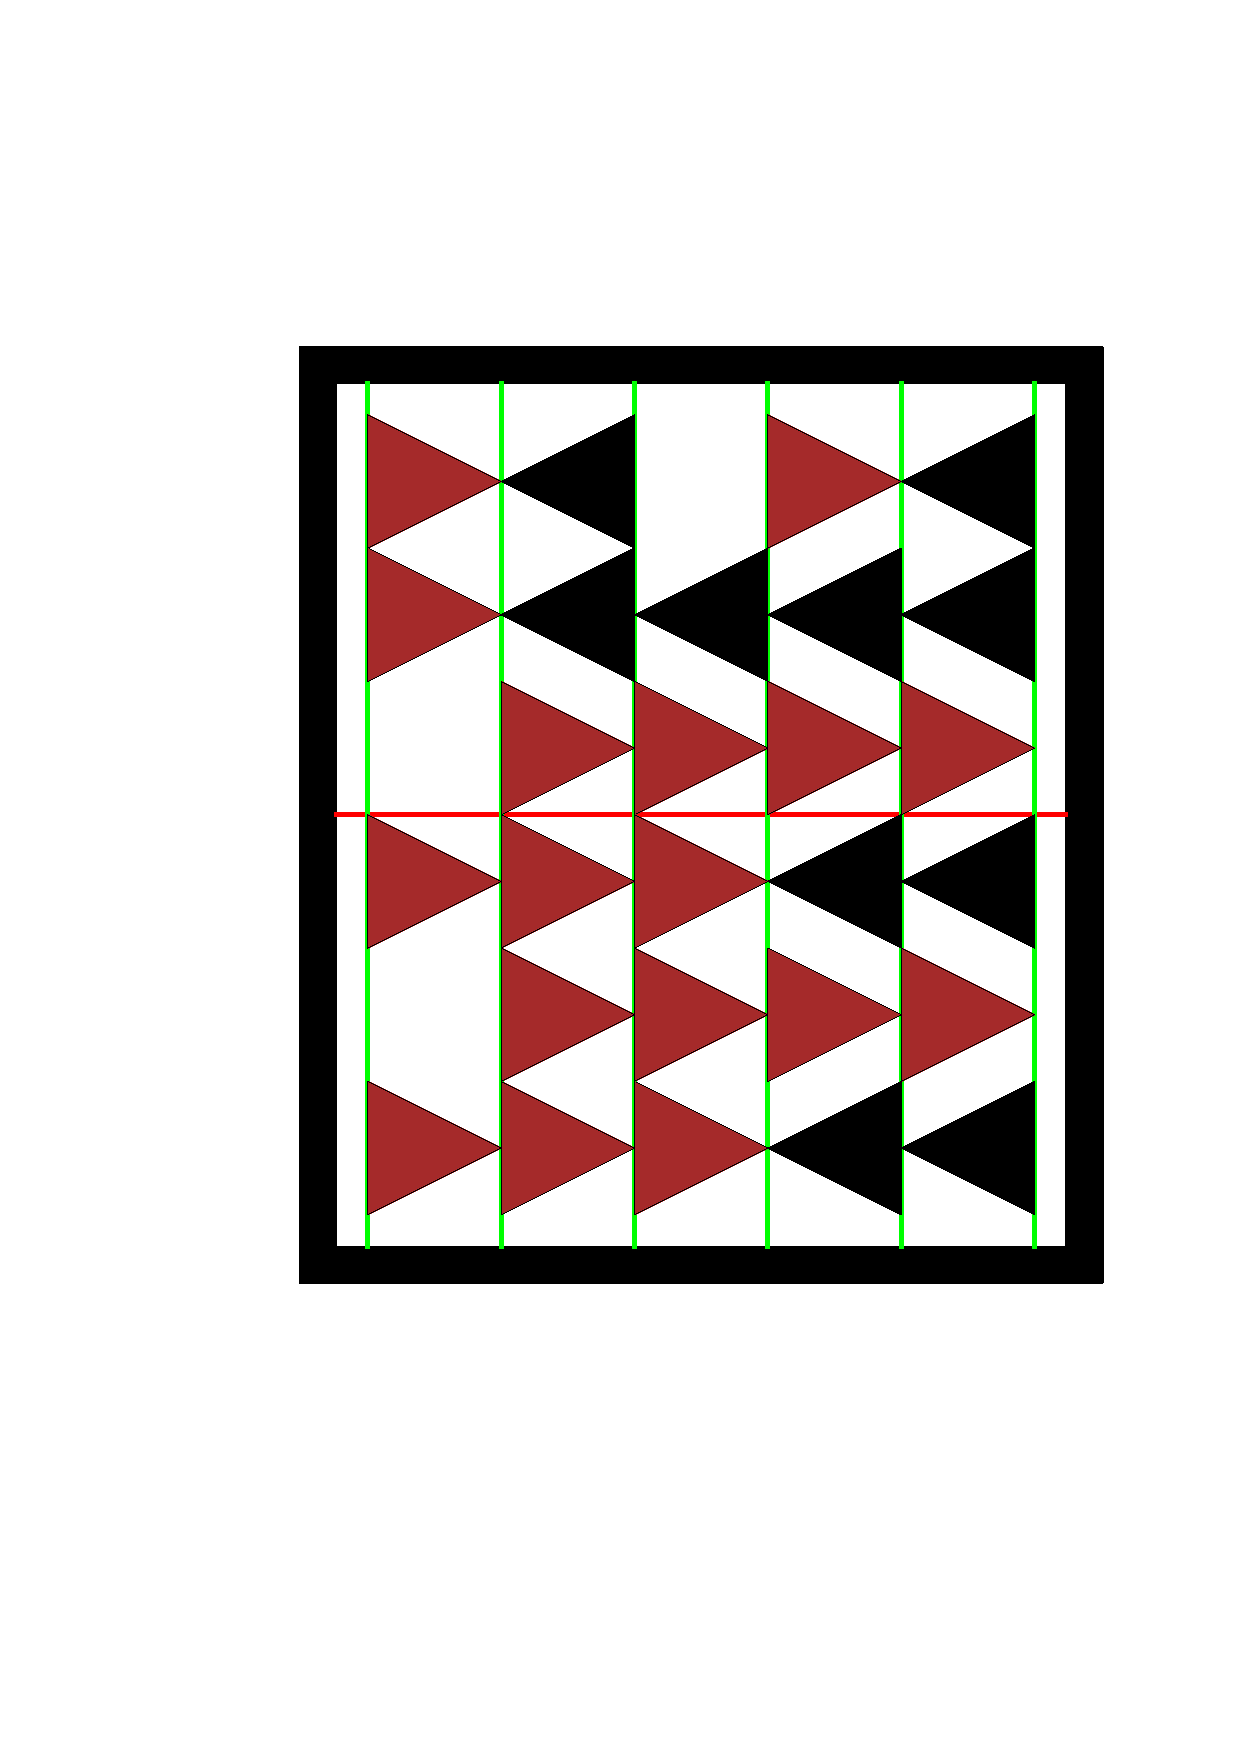
\includegraphics{graphics/LogicEngineFrameFigure5.pdf}
\caption{The logic engine from figure \ref{fig:LogicEngineFrameFigure2.pdf} whose armatures are rotated}\label{fig:LogicEngineFrameFigure5.pdf}
\end{center}
\end{figure}
\begin{thm}\label{thm:Satisfiability-1}
 Given an instance of $NAE3SAT$,  it is a ``yes'' instance if and only if the 
corresponding logic engine has a flat, collision-free configuration.
\end{thm}
\begin{proof}
 %  If an instance of $NAE3SAT$ is a ``yes'', then every clause in $C$ contains at least one true
% variable and one false variable.  
Suppose that the $NAE3SAT$ is a ``yes'' instance.  This implies that each clause each clause contains a 
true and false literal.  Each clause has a pair of corresponding rows in the logic engine, one row for non-negated literals and one for negated literals.  If the literal exists in the clause, then it is unflagged in that corresponding row.  The flagged literals shall point towards the nearest unflagged literal in each row.  Each row is collision free since adjacent flags will either be in the (left, left), (right, right), or (left, right) position as shown in figure \ref{fig:logicEngineValidConfigurations.pdf}.  If the logic engine is collision-free, then the engine and be made flat and remain collision-free and so the corresponding logic engine has a flat collision-free configuration.

Given the corresponding logic engine has a flat, collision-free configuration for a $NAE3SAT$ instance.  Then every row must have an unflagged armature.  Each clause has two corresponding rows, one row for negated literals and one for non-negated literals.  Unflagged armatures implies the existence of a literal in a clause. All together, this implies that every clause contains a true and false literal.  Thus we have a ``yes'' $NAE3SAT$ instance.
\end{proof}

\subsection{Construction of the NAE3SAT Problem over Hinged Polygons}

\subsection{Construction of the NAE3SAT Problem over Disks}
